\documentclass[class=book, crop=false]{standalone}
\usepackage[subpreambles=true]{standalone}

\usepackage{../../style}

\graphicspath{{./assets/images/}}

\begin{document}
\chapter{Le reti logiche}
\section{Introduzione}
Come ben sappiamo, a differenza di \emph{ENIAC}, i computer moderni sono realizzati da un'enorme quantità di circuiti elettronici. Trattandosi di eletronica digitale, a livello hardware è possibile lavorare con due livelli fondamentali:
\begin{itemize}[noitemsep, nolistsep]
	\item 1: alto, asserito; associato alla tensione di alimentazione \emph{Vdd}.
	\item 0: basso, negati; associato alla massa (tensione vicina a 0).
\end{itemize}
Nel passaggio da un livello all'altro si presenta lo stato \emph{transitorio}, in cui la tensione assume valori intermedi fra zero e Vdd.\\
In particolare, i \textbf{circuiti logici} (formati dalle \textbf{porte logiche}) vengono utilizzati per trasformare alcuni valori logici in ingresso in altri valori logici in uscita. I circuiti logici si differenziano principalmente in:
\begin{itemize}[nolistsep, noitemsep]
	\item \emph{Combinatorie}: l'uscita dipende unicamente dal valore di ingresso (non sono dotati di memoria).
	\item \emph{Sequenziali}: l'uscita dipende dal valore di ingresso e dalla storia degli ingressi precedenti (sono dotati di memoria, detta "stato" della rete).
\end{itemize}
\`{E} possibile riassumere il comportamento di una rete logica attraverso una \emph{tabella di verità}, che descrive i diversi output al variare dei diversi input.

\section{L'algebra di Boole}
Esisotno principalmente tre operazioni di base:
\begin{itemize}[noitemsep, nolistsep]
	\item \textbf{AND}: \(A\cdot B\); produce 1 se entrambi gli operandi sono 1, 0 altrimenti.
	\item \textbf{OR}: \(A+B\); produce 0 se entrambi gli operandi sono 0, 1 altrimenti.
	\item \textbf{NOT}: \(\overline{A}\); inverte il valore logico.
\end{itemize}
\subsection{Regole di semplificazione}
\label{subsec:semplificazione}
Di seguito vengono riportate alcune regole di semplificazione:
\begin{itemize}
	\item Identità: \(A+0=A\), \(A\cdot 1=A\)
	\item Regola "zero e uno": \(A+1=1\), \(A\cdot 0=0\)
	\item Regola dell'inversa: \(A+\overline{A}=1\), \(A\cdot\overline{A}=0\)
	\item Regola commutativa: \(A+B=B+A\), \(A\cdot B=B\cdot A\)
	\item Regola associativa: \(A+(B+C)=(A+B)+C\), \(A\cdot(B\cdot C)=(A\cdot B)\cdot C\)
	\item Regola distributiva: \(A\cdot(B+C)=(A\cdot B)+(A\cdot C)\), \(A+(B\cdot C)=(A+B)\cdot(A+C)\)
	\item De Morgan: \(\overline{A\cdot B} = \overline{A}+\overline{B}\), \(\overline{A+B} = \overline{A}\cdot\overline{B}\)
\end{itemize}
Proprio grazie alla regola di De Morgan, si può affermare che la porta \textbf{NAND} (not AND) e la porta \textbf{NOR} (not OR) sono universali. Ciò significa che utilizzando unicamente porte NAND (rispettivamente NOR) è possibile costruire tutte le altre porte logiche.
\subsection{La tavola di verità e i mintermini}
\label{subsec:mintermini}
\begin{table}[!h]
	\centering
	\subimport{assets/tables/}{tabella_verita}
	\caption{Esempio di tabella di verità}
	\label{tabella-verita}
\end{table}
Si può verificare che:
\begin{gather*}
D = A+B+C\\
F = A\cdot B\cdot C\\
E = (A\cdot B\cdot\overline{C}) + (A\cdot C\cdot\overline{B}) + (B\cdot C\cdot\overline{A})
\end{gather*}
In particolare, l'ultima espressione è stata ottenuta come somme di prodotti attraverso i cosiddetti \emph{mintermini}. Per ciscun 1 presente nella colonna E, si scrive il prodotto degli input (asseriti se pari a 1, negati se pari a 0); il risultato dell'espressione è pari alla somma di tali prodotti.

\section{Le porte logiche}
A seguire vengono rappresentate, attraverso i corrispettivi simboli, le porte logiche implementate attraverso gli operatori booleani fondamentali:
\begin{figure}[H]
	\centering
	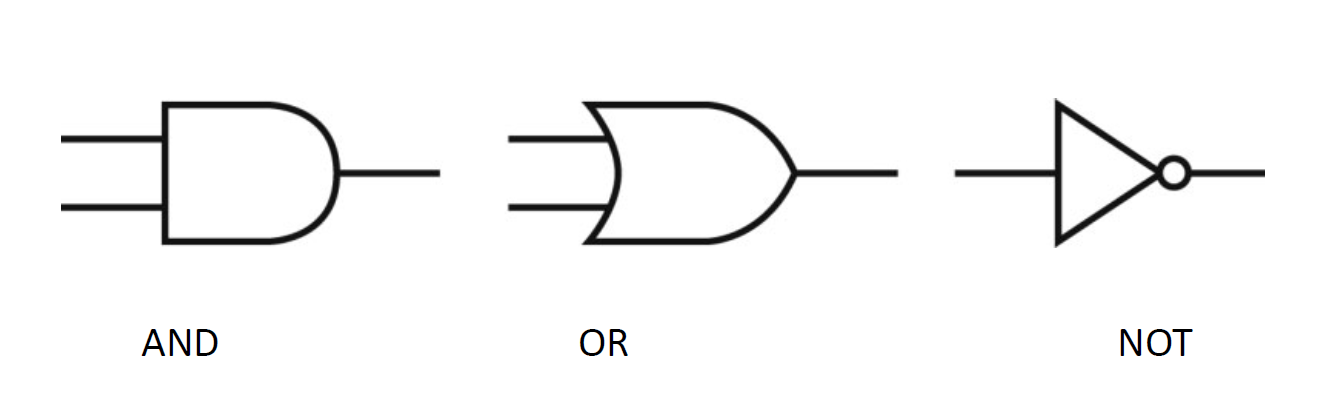
\includegraphics[width=0.8\textwidth,keepaspectratio]{porte_logiche.png}
	\caption{Rappresentazione di AND, OR e NOT}
\end{figure}

Si ricorda inoltre che è possibile combinare fra loro diverse porte logiche:
\begin{figure}[H]
	\centering
	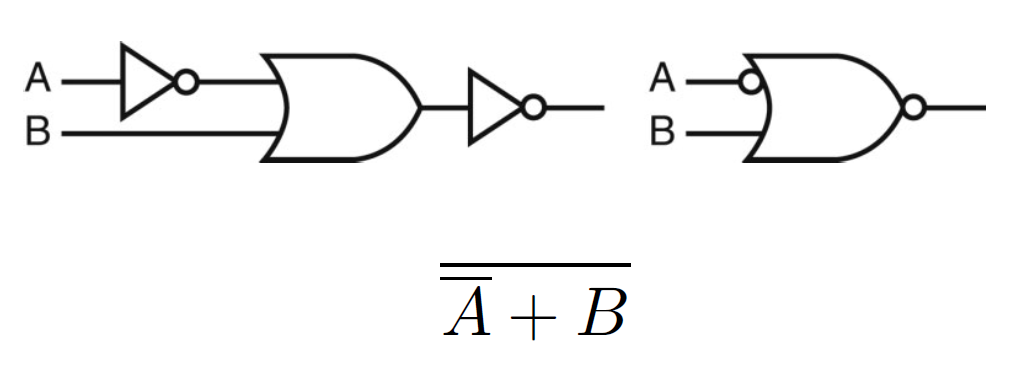
\includegraphics[width=0.8\textwidth,keepaspectratio]{combinazione_porte.png}
	\caption{Combinazione di porte logiche}
\end{figure}

\section{Alcuni circuiti degni di nota}
\subsection{Decoder}
L'ingresso del \emph{decoder} svolge il ruolo di selettore: ricevendo in input il valore \(n\), si accenderà l'\(n\)-esima uscita. A seguire l'implementazione di un decoder a 3 bit:
\begin{figure}[H]
	\centering
	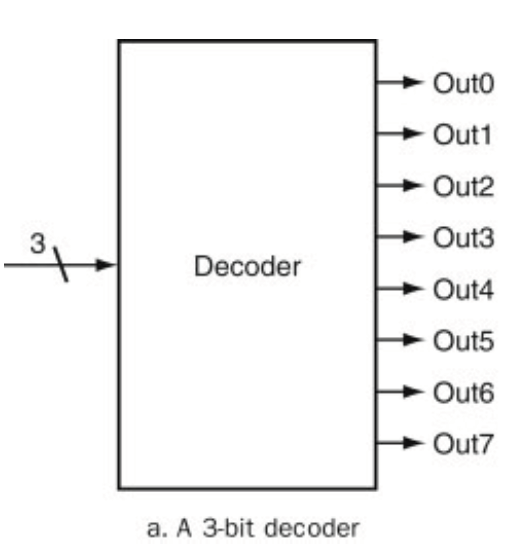
\includegraphics[width=0.4\textwidth,keepaspectratio]{3bit_decoder.png}
	\caption{Decoder a 3 bit}
\end{figure}
\begin{table}[!h]
	\centering
	\begin{tabular}{|c|c|c|c|c|c|c|c|c|c|c|}
		\hline
		\rowcolor[HTML]{EFEFEF}
		\multicolumn{3}{|c|}{\cellcolor[HTML]{EFEFEF}Input} & \multicolumn{8}{c|}{\cellcolor[HTML]{EFEFEF}Output} \\ \hline
		\rowcolor[HTML]{EFEFEF}
		In2 & In1 & In0 & Out7 & Out6 & Out5 & Out4 & Out3 & Out2 & Out1 & Out0 \\ \hline
		0 & 0 & 0 & 0 & 0 & 0 & 0 & 0 & 0 & 0 & 1 \\ \hline
		0 & 0 & 1 & 0 & 0 & 0 & 0 & 0 & 0 & 1 & 0 \\ \hline
		0 & 1 & 0 & 0 & 0 & 0 & 0 & 0 & 1 & 0 & 0 \\ \hline
		0 & 1 & 1 & 0 & 0 & 0 & 0 & 1 & 0 & 0 & 0 \\ \hline
		1 & 0 & 0 & 0 & 0 & 0 & 1 & 0 & 0 & 0 & 0 \\ \hline
		1 & 0 & 1 & 0 & 0 & 1 & 0 & 0 & 0 & 0 & 0 \\ \hline
		1 & 1 & 0 & 0 & 1 & 0 & 0 & 0 & 0 & 0 & 0 \\ \hline
		1 & 1 & 1 & 1 & 0 & 0 & 0 & 0 & 0 & 0 & 0 \\ \hline
	\end{tabular}
	\caption{Tabella di verità per un decoder a 3 bit}
	\label{decoder-3bit}
\end{table}

\subsection{Multiplexer}
Prevede un input con valore \(S\) utilizzato come selettore. L'output del \emph{multiplexer} è il valore dell'input \(S\)-esimo.
\begin{figure}[H]
	\centering
	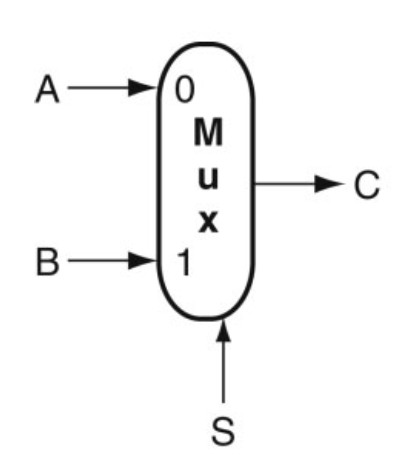
\includegraphics[width=0.3\textwidth,keepaspectratio]{multi.png}
	\caption{Multiplexer a 1 bit}
\end{figure}
\`{E} possibile costruire un multiplexer attraverso un decoder:
\begin{figure}[H]
	\centering
	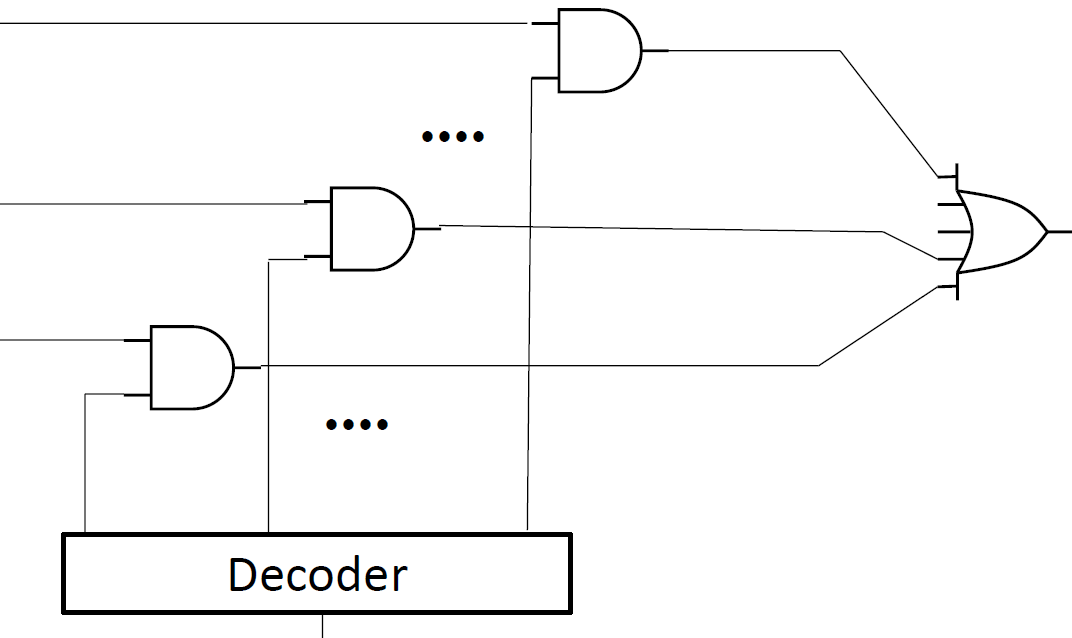
\includegraphics[width=0.7\textwidth,keepaspectratio]{multi_n_vie.png}
	\caption{Multiplexer a n vie}
\end{figure}
Molto spesso, per operare con dati complessi, si compongono degli array di elementi elementari. Segue un esempio di come sia possibile costruire un multiplexer con \emph{bus} a 32 bit utilizzando un array di multiplexer a 1 bit.
\begin{figure}[H]
	\centering
	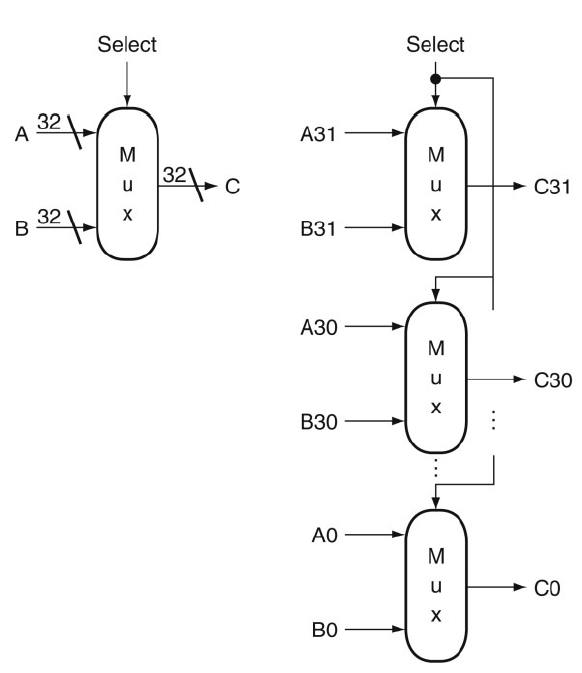
\includegraphics[width=0.7\textwidth,keepaspectratio]{mux_32bit.png}
	\caption{Multiplexer a 32 bit}
\end{figure}

\subsection{Programmable Logic Array (PLA)}
Il \emph{programmable logic array} si compone di due strutture: una barriera di AND e da una barriera di OR. La dimensione totale del \emph{PLA} è data dalla somma del piano AND (numero di mintermini) e del piano OR (numero di uscite).\\
Inoltre, il PLA implementa porte logiche solamente per le configurazioni che producono 1 in uscita. In aggiunta, se un mintermine è condiviso tra varie uscite, lo si può riutilizzare.
Successivamente seguono due diverse implementazioni della rete logica descritta nel paragrafo~\ref{subsec:mintermini}.
\begin{figure}[H]
	\centering
	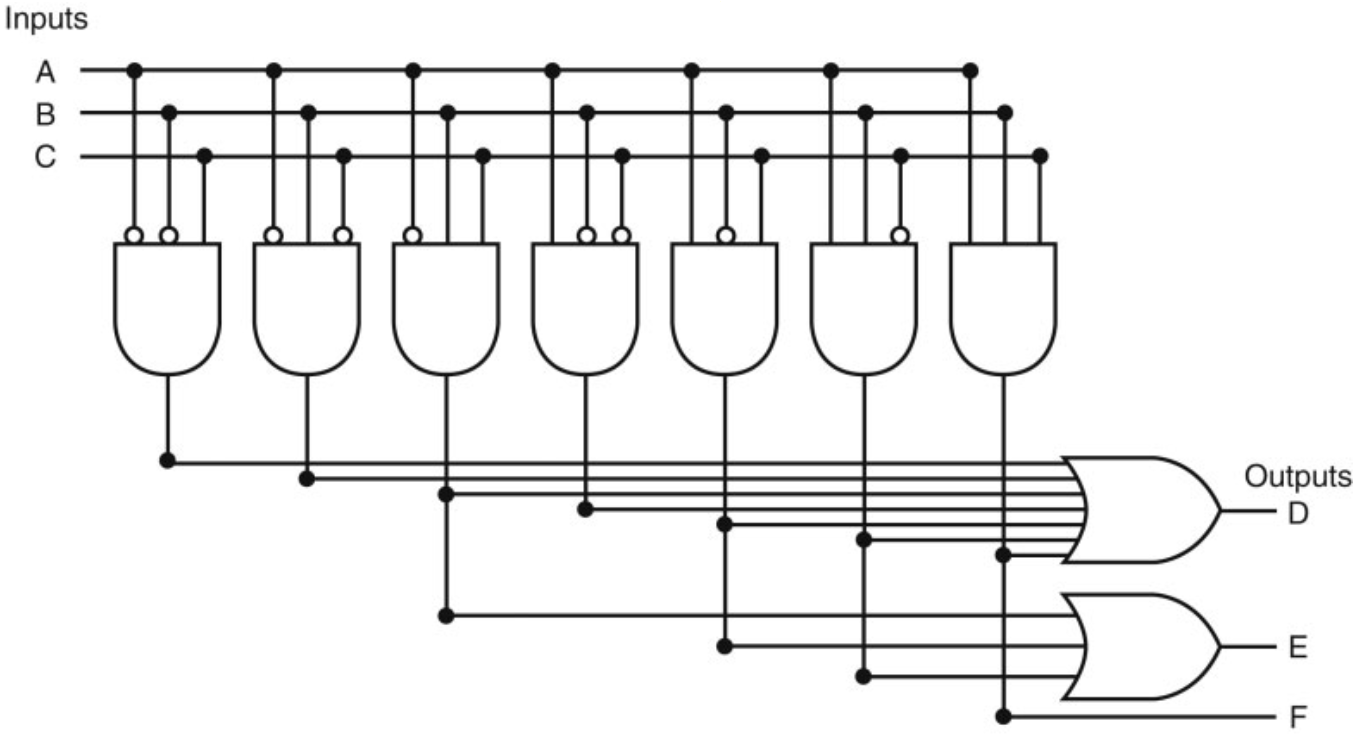
\includegraphics[width=0.7\textwidth,keepaspectratio]{es_rete_logica.png}
	\caption{Esempio di rete logica}
\end{figure}
\begin{figure}[H]
	\centering
	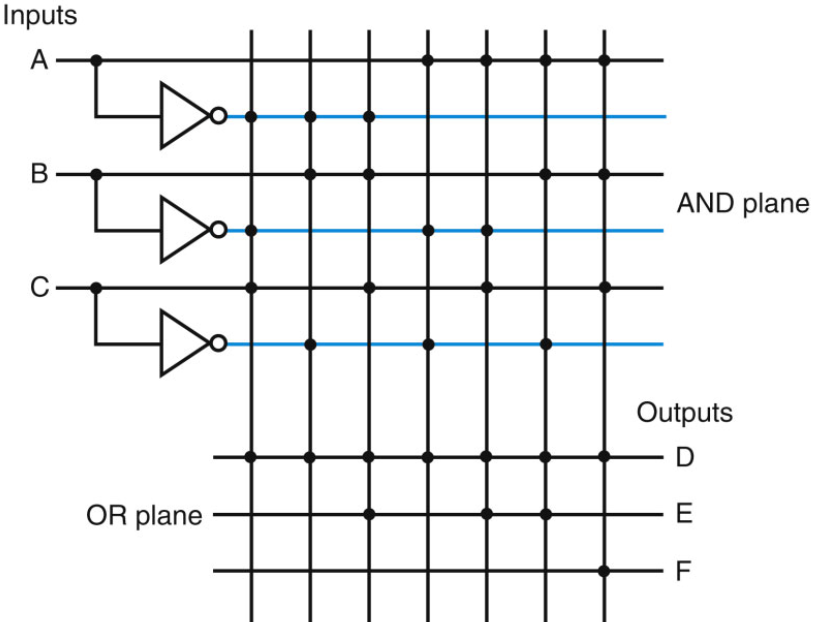
\includegraphics[width=0.7\textwidth,keepaspectratio]{es_pla.png}
	\caption{Esempio di rete logica implementata attraverso PLA}
\end{figure}

\section{Il concetto di \emph{costo}}
Come appena visto, le reti logiche possono essere implementate in maniera differente. Si definisce \emph{costo} di una rete logica la somma del numero di porte e del numero di ingressi della rete. Quando si analizza una rete, è importante saperne trovare l'implementazione con costo minimo. Principalmente si può procedere in due modalità:
\begin{itemize}[noitemsep]
	\item regole di semplificazione matematiche dovute all'algebra di Boole (vedi paragrafo~\ref{subsec:semplificazione}).
	\item metodi basati su rappresentazioni grafiche (mappe di \emph{Karnaugh}), nei casi più semplici.
\end{itemize}

\section{Le reti sequenziali}
Come si è visto, le reti combinatorie non hanno memoria degli stati del passato: in ogni istante di tempo l’uscita dipende solamente dagli ingressi nell’istante considerato. Tuttavia, in certe applicazioni è necessario introdurre una vera e propria memoria nel sistema.\\
La memoria in una rete logica si ottiene attraverso una \emph{retroazione}, che consiste nel ridirezionare alcune porte di uscita in ingresso ad altre porte del medesimo circuito, in maniera tale da formare un anello.\\
Seppur questo meccanismo offra delle potenzialità enormi, l'analisi e la sintesi di una rete logica è molto più complessa rispetto a quella delle reti combinatorie.

\subsection{Latch S-R}
A seguire un'implementazione di una rete sequenziale \emph{latch S-R} (\emph{set-reset}) costruita attraverso due porte NOR:
\begin{figure}[H]
	\centering
	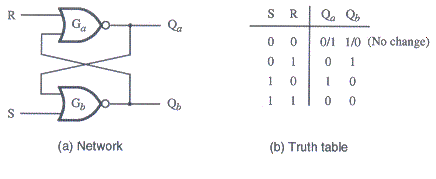
\includegraphics[width=0.8\textwidth,keepaspectratio]{es_latch.png}
	\caption{Esempio di latch a porte NOR}
\end{figure}
\begin{figure}[H]
	\centering
	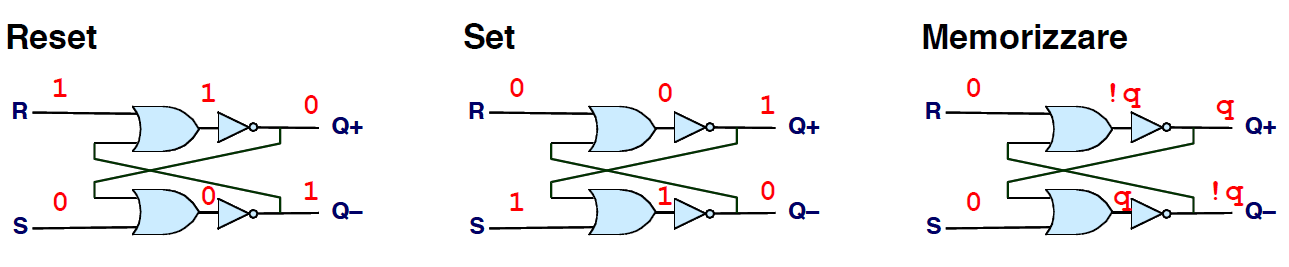
\includegraphics[width=\textwidth,keepaspectratio]{operazioni_latch.png}
	\caption{Operazioni di un latch a porte NOR}
\end{figure}
Ma, considerando che i segnali non si propagano in tempo nullo, ciò potrebbe causare dei problemi circa la correttezza del segnale stesso. La soluzione è quella di aggiungere un ulteriore segnale, in grado di temporizzare il circuito: il \emph{clock}. Un latch dotato di temporizzazione viene chiamato \emph{gated latch}.
\begin{figure}[H]
	\centering
	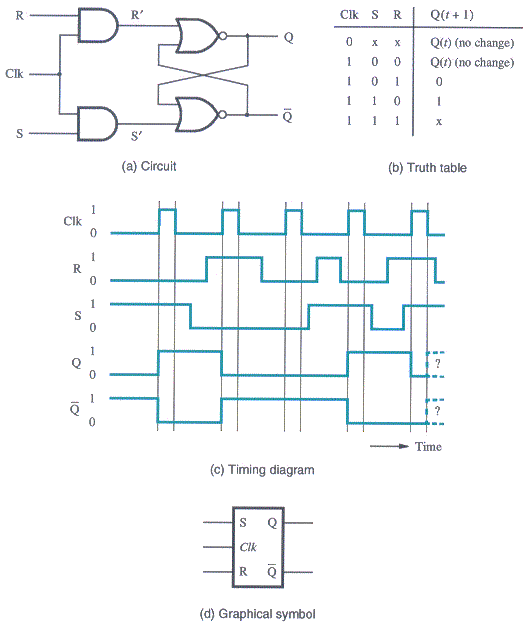
\includegraphics[width=\textwidth,keepaspectratio]{gated_latch.png}
	\caption{Esempio di gated latch}
\end{figure}
Il difetto principale di un latch R-S è quello di avere uno stato indecidibile: l'uscita non può essere nota con certezza quando entrambi gli ingressi sono a 1.

Una soluzione è implementata attraverso \emph{latch} tipo \emph{D}: gli ingressi al circuito sono ottenuti da un'unica variabile (di cui se ne fa il negato). Altrimenti, attraverso circuiti \emph{flip-flop master-slave} è possibile ottenere che l’uscita del circuito commuti esattamente al termine dell’impulso di clock.\\
In particolare, i latch di tipo D vengono utilizzati per implementare i registri della CPU.

\end{document}
